\chapter{Σχετική Βιβλιογραφία}
\label{ch:related_work}
Τα ερωτήματα εγγύτητας και η ανίχνευση σύγκρουσης διερευνώνται 
εκτενώς για δεκαετίες από ερευνητές στα γραφικά υπολογιστών, στη ρομποτική,
στις προσομοίωσες, την υπολογιστική γεωμετρία και τα κινούμενα σχέδια 
υπολογιστών. 
Εκτός από την ανίχνευση σύγκρουσης και τον υπολογισμό απόστασης, υπάρχει
σημαντική βιβλιογραφία σχετική με τις Ιεραρχίες Οριοθετικών Όγκων 
(\tl{BVH}) και τις διάφορες εφαρμογές τους. 
Σε αυτό το κεφάλαιο κάνουμε αναφορά σε άρθρα της βιβλιογραφίας 
που μελετούν το ίδιο ή παρόμοιο πρόβλημα με το δικό μας
και επισημαίνουμε τις τεχνικές που χρησιμοποιούνται 
και στη δική μας μεθοδολογία.

\section{Εύρεση Κοντινότερου Κόμβου από Σημείο}
Αρχικά μελετάμε το παρακάτω πρόβλημα: \textit{"Δοθέντος ενός 
πλέγματος και ενός σημείου (\tl{query-point}), ζητείται να βρεθεί 
ο κοντινότερος προς το σημείο \textbf{κόμβος} του πλέγματος"}.
Το πρόβλημα αυτό ανάγεται στο κλασικό πρόβλημα εύρεσης των \textit{$k$ 
κοντινότερων γειτόνων} από ένα σύνολο σημείων (\tl{$k$NN}, όπου $k=1$). 

Για το πρόβλημα αυτό έχουν προταθεί διάφορες λύσεις. Για παράδειγμα 
η χρήση διαγραμμάτων \tl{Voronoi} στην περίπτωση δεδομένων 
με μικρό αριθμό διαστάσεων \cite{aurenhammer1991voronoi}.
Οι σημαντικότερες όμως συνεισφορές για το συγκεκριμένο πρόβλημα είναι 
αυτές του \cite{bentley1975multidimensional} με την εισαγωγή του 
\textit{\tl{kD-Tree}}, και του \cite{yianilos1993data} με την 
εισαγωγή του \textit{\tl{VP-Tree}} (βλ. για παράδειγμα το
\cite{simon1996fast} όπου γίνεται χρήση του \textit{\tl{kD-Tree}} για τον 
υπολογισμό του κοντινότερου κόμβου ενός τριγωνικού πλέγματος 
από σημείο).

Τα δύο παραπάνω δυαδικά δέντρα αναζήτησης απαιτούν $\bigO(n*logn)$
χρόνο προεπεξεργασίας των δεδομένων (για την κατασκευή τους
από το σύνολο των $n$ σημείων του τρισδιάστατου χώρου) και 
έπειτα $\bigO(logn)$ για την απάντηση ερωτημάτων κοντινότερου 
γείτονα, στη μέση περίπτωση. 
Στο ίδιο πλαίσιο εργασίας αναπτύσσεται ο πρώτος εκ των δύο αλγορίθμων που 
προτείνουμε, για το δικό μας πρόβλημα, όπου κατασκευάζουμε μια δομή 
δεδομένων και στη συνέχεια κάνουμε ερωτήματα κοντινότερου γείτονα 
για να υπολογίσουμε την απόσταση.

Πιο συγκεκριμένα, για την κατασκευή του \tl{\textit{kD-Tree}} το σύνολο 
των σημείων ενός κόμβου διχοτομείται σε δύο υποσύνολα που αποτελούν 
τα δύο παιδιά του κόμβου. Η διαδικασία αυτή επαναλαμβάνεται αναδρομικά:
\begin{itemize}
    \item Η διχοτόμηση γίνεται με βάση κάποιον άξονα ο οποίος εναλλάσσεται κυκλικά 
    (\tl{round-robin}) για τα διαδοχικά επίπεδα του δέντρου.
    Για παράδειγμα, στις τρεις διαστάσεις, ο διαχωρισμός γίνεται πρώτα με 
    βάση τον άξονα $x$, έπειτα με βάση τον άξονα $y$, έπειτα με τον $z$, 
    ξανά με βάση τον $x$ και ούτω καθεξής.
    \item Το κριτήριο για τον διαχωρισμό του συνόλου των σημείων $V$, ενός κόμβου, 
    σε δύο υποσύνολα $L$, $R$ είναι το εξής: Χωρίς βλάβη της γενικότητας 
    θεωρούμε πως ο άξονας διαχωρισμού είναι ο $x$. Αν $m$ είναι η διάμεσος 
    των $x$-συντεταγμένων των σημείων, τότε $L = \{p \in V \mid p_x \leq m \}$ 
    και $R = \{p \in V \mid p_x >= m \}$. 
    Τα σύνολα $L$, $R$ επιλέγονται ώστε να έχουν το ίδιο πλήθος στοιχείων 
    ή να διαφέρουν κατά ένα.
    Όμοια προκύπτει το κριτήριο και για τους άλλους άξονες.
    Η διάμεσος $m$ είναι πληροφορία που αποθηκεύεται για κάθε κόμβο του δέντρου
    και χρησιμοποιείται στα ερωτήματα εύρεσης του κοντινότερου γείτονα.
\end{itemize}

Έτσι προκύπτει ένα σχεδόν πλήρες, ισορροπημένο, δυαδικό δέντρο.
Οι ιδέες 1) της διχοτόμησης του συνόλου των δεδομένων με κυκλική εναλλαγή 
του άξονα διαχωρισμού και 2) η χρήση της διαμέσου των αντίστοιχων 
συντεταγμένων για τον διαχωρισμό  
χρησιμοποιούνται \textit{αυτούσιες} και στη δική μας μεθοδολογία 
για την κατασκευή μιας Ιεραρχίας Οριοθετικών Όγκων. 
Η διαφορά είναι πως χειριζόμαστε χωρικά δεδομένα, και όχι σημεία,
επομένως επιλέγεται ένα \textit{αντιπροσωπευτικό σημείο} για κάθε 
χωρικό αντικείμενο και εφαρμόζεται η ίδια μέθοδος κατασκευής της 
ιεραρχίας. 

\begin{wrapfigure}{l}{0.3\textwidth}
    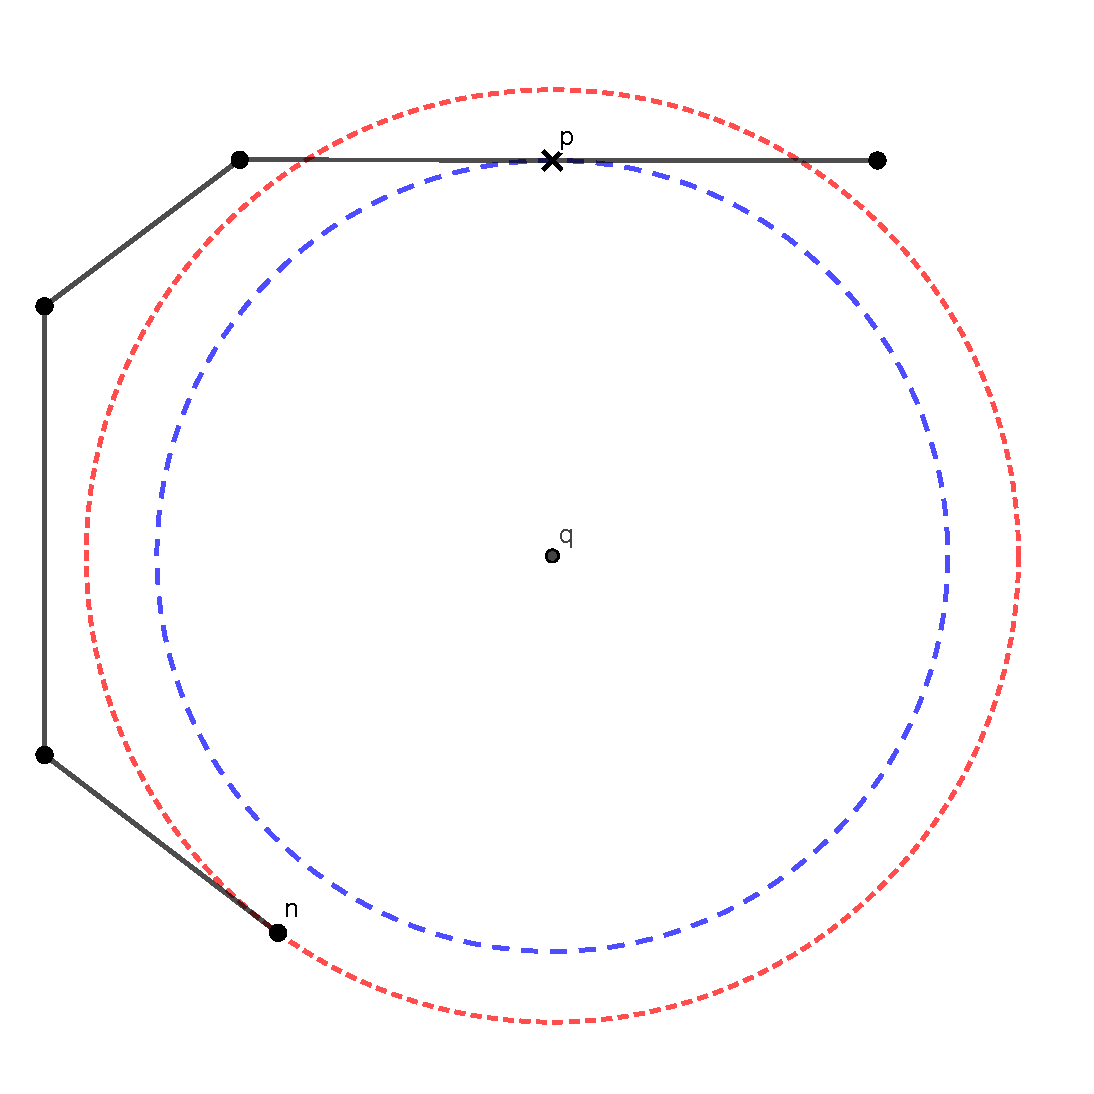
\includegraphics[width=0.29\textwidth]{nearest_node.pdf}
    \caption[Εύρεση Κοντινότερου Κόμβου από Σημείο]{
        Παράδειγμα όπου ο κοντινότερος \textit{κόμβος} $n$ ενός πλέγματος 
        διαφέρει από το κοντινότερο \textit{σημείο} $p$, δοθέντος 
        του \tl{query-point} $q$.}
    \label{fig:nearest_node}
\end{wrapfigure}

Για την κατασκευή του \tl{\textit{VP-Tree}}, ξανά, το σύνολο των σημείων 
ενός κόμβου διχοτομείται σε δύο υποσύνολα αναδρομικά:
\begin{itemize}
    \item Αρχικά, επιλέγεται ένα τυχαίο σημείο από το σύνολο $V$ των σημείων 
    του κόμβου. Το σημείο αυτό ονομάζεται \textit{\tl{vantage-point (vp)}} 
    και αποτελεί πληροφορία που αποθηκεύεται στον κόμβο.
    \item Έπειτα υπολογίζονται οι αποστάσεις όλων των υπολοίπων σημείων 
    προς το \tl{vp} και η διάμεσος $m$, που επίσης αποθηκεύεται στον κόμβο.
    \item Αν $m$ είναι η διάμεσος των αποστάσεων που υπολογίστηκαν 
    τότε το σύνολο του αριστερού παιδιού είναι το 
    $L = \{p \in V \mid distance(p,vp) \leq m \}$
    και του δεξιού παιδιού 
    $R = \{p \in V \mid distance(p,vp) \geq m \}$
\end{itemize} 

Ο τυπικός τρόπος για την απάντηση ερωτημάτων κοντινότερου κόμβου 
είναι, αρχικά, ο υπολογισμός μιας εκτίμησης αυτού διασχίζοντας το δέντρο 
από τη ρίζα έως κάποιο φύλλο. 
Το φύλλο αποτελεί την πρώτη εκτίμηση κοντινότερου κόμβου, ενώ η επιλογή του 
μονοπατιού από τη ρίζα μέχρι το φύλλο αποτελεί σχεδιαστική επιλογή και 
χρησιμοποιούνται ευρετικοί μέθοδοι (\tl{heuristics}).
Έπειτα μια σφαίρα εκτείνεται από το \tl{query-point} έως το φύλλο 
και, με τη βοήθεια του δέντρου, από τα υπόλοιπα σημεία ελέγχονται μόνο 
αυτά που βρίσκονται εντός της σφαίρας. 
Η ακτίνα της σφαίρας μικραίνει όσο ανακαλύπτονται όλο και κοντινότεροι 
κόμβοι.
Αυτή η διαδικασία λέγεται \textit{κλάδεμα (\tl{pruning})} του δέντρου,
και μειώνει τον χώρο αναζήτησης με το να απορρίπτει περιοχές που δεν 
μπορούν να περιέχουν τον κοντινότερο γείτονα. 
Με αυτόν τον τρόπο, ο αριθμός των αναμενόμενων συγκρίσεων 
είναι της τάξης $\bigO(logn)$ για τη μέση περίπτωση. 
Με ίδιο μοτίβο λογικής σχεδιάζεται και η διαδικασία αναζήτησης 
κοντινότερου γείτονα για χωρικά δεδομένα που προτείνουμε. 

Το παραπάνω πρόβλημα δεν πρέπει να συγχέεται με το πρόβλημα εύρεσης 
του κοντινότερου \textit{σημείου} ενός πολυγωνικού πλέγματος από 
κάποιο \tl{query-point}. Γενικά ο κοντινότερος \textit{κόμβος} και 
το κοντινότερο \textit{σημείο} ενός πλέγματος μπορούν να απέχουν 
πολύ μεταξύ τους όπως φαίνεται στο Σχήμα \ref{fig:nearest_node}:
Η πολυγωνική γραμμή αντιπροσωπεύει το σύνορο ενός υποθετικού πλέγματος 
στις δύο διαστάσεις και η ελάχιστη απόσταση του πλέγματος από το σημείο 
$q$ (ακτίνα του κόκκινου κύκλου) διαφέρει από την 
απόσταση του κοντινότερου κόμβου (ακτίνα του μπλε κύκλου).



\section{Ανίχνευση Σύγκρουσης και Υπολογισμός Απόστασης Κυρτών Πολυγώνων}
% να πω για linear programming 
% These include Dobkin-
% Kirkpatrick hierarchies [DK82], linear programming [Sei90] and algorithms for intersecting
% convex p olytop es [Cha89 ] 
% και γενικά ό,τι αναφέρεται στο paper του GJK.

\section{Ιεραρχικές Δομές Δεδομένων}
%να αναφέρω SAH
%R-Trees
%BSP Trees
% Απόσταση Σημείου από Πολυγωνικό Πλέγμα
% Απόσταση Δύο Πολυγωνικών Πλεγμάτων
% Απόσταση Αντικειμένων που Περιγράφονται από \tl{NURBS}
